% ============================================================
%  Chapter 1 — The Family of Vehicle Routing Problems
%  Self-contained Beamer slides (reader-friendly, no presenter needed)
%  Source: Irnich, Toth, Vigo in "Vehicle Routing: Problems, Methods,
%          and Applications", 2nd ed., SIAM, 2014.
%  Authors of chapter: Stefan Irnich, Paolo Toth, Daniele Vigo
% ============================================================
\documentclass[aspectratio=169,10pt]{beamer}

\usetheme{Madrid}
\usecolortheme{seahorse}

\usepackage{amsmath,amssymb,amsfonts}
\usepackage{graphicx}
\usepackage{booktabs}
\usepackage{xcolor}
\usepackage{listings}
\usepackage{tikz}
\usepackage{array}
\usepackage{multirow}
\usepackage{microtype}
\usepackage{hyperref}

\graphicspath{{figures/}}

\setbeamertemplate{footline}[frame number]
\setbeamertemplate{navigation symbols}{}

% Python listings style
\lstset{
  language=Python,
  basicstyle=\ttfamily\scriptsize,
  numbers=left,
  numberstyle=\tiny\color{gray},
  frame=single,
  backgroundcolor=\color{gray!7},
  commentstyle=\color{green!50!black}\itshape,
  keywordstyle=\color{blue!70!black}\bfseries,
  stringstyle=\color{red!60!black},
  breaklines=true,
  showstringspaces=false,
  tabsize=4,
}

% ─── Title ──────────────────────────────────────────────────────────────────
\title[The Family of VRP]{%
  Chapter 1: The Family of Vehicle Routing Problems}
\subtitle{Vehicle Routing: Problems, Methods, and Applications\\
          2nd Edition, SIAM, 2014}
\author{Stefan Irnich \and Paolo Toth \and Daniele Vigo\\[4pt]
  \small Slides compiled for self-study}
\date{2014 (slides prepared 2026)}

% ============================================================
\begin{document}
% ============================================================

\begin{frame}
  \titlepage
\end{frame}

\begin{frame}{Table of Contents}
  \tableofcontents
\end{frame}

% ============================================================
\section{1.1 Introduction}
% ============================================================

\begin{frame}[allowframebreaks]{What Is the Vehicle Routing Problem?}

The \textbf{Vehicle Routing Problem (VRP)} is one of the most studied problems in
combinatorial optimisation, with widespread real-world applications in logistics,
distribution, and transportation.  A precise verbal definition is the following:

\begin{block}{Informal Definition of the VRP (Irnich, Toth, Vigo 2014)}
\textbf{Given:} A set of \emph{transportation requests} and a \emph{fleet of vehicles}.\\[4pt]
\textbf{Task:} Determine a set of \emph{vehicle routes} to \emph{perform} all (or some)
transportation requests with the given vehicle fleet \emph{at minimum cost}.  In
particular, decide \emph{which vehicle handles which requests in which sequence} so that
all vehicle routes can be \emph{feasibly} executed.
\end{block}

In this type of problem the transportation requests to be served are generally
concentrated in specific \emph{points} of a road network.  This contrasts with the
\emph{Arc Routing Problems} (ARP), where requests are dispersed along the arcs, i.e.,
street segments of the underlying road network.

\medskip
The four key components of any VRP instance are:
\begin{enumerate}
  \item \textbf{Transportation requests} --- what needs to be moved, and where.
  \item \textbf{Fleet of vehicles} --- how many vehicles, of what type, from what depot.
  \item \textbf{Costs} --- travel distance, time, fuel, driver wages, etc.
  \item \textbf{Feasibility of routes} --- physical constraints (capacity, hours, time windows).
\end{enumerate}

\framebreak

\begin{alertblock}{Economic Relevance}
The large number of real-world applications have widely shown that the use of
computerised solution methods for the VRP, both at the planning and the operational
levels, yields \emph{substantial savings} in global transportation costs.  The success
of optimisation techniques is due not only to the power of modern computer systems
and the full integration of information systems into operations, but also to the
development of rigorous mathematical models that can take into account almost all
characteristics of real-world distribution processes.
\end{alertblock}

\medskip
The chapter also serves as a foundation for the research on specific VRP variants
described in later chapters.  It presents basic models, identifies the main
components that distinguish variants from each other, and provides a taxonomy of the
VRP family.

\end{frame}

% ============================================================
\section{1.2 The Capacitated Vehicle Routing Problem (CVRP)}
% ============================================================

\begin{frame}[allowframebreaks]{1.2.1 Problem Statement}

The \textbf{Capacitated Vehicle Routing Problem (CVRP)} is the most fundamental
and most-studied member of the VRP family.  Every other variant can be understood as
the CVRP with additional constraints or relaxations.

\begin{block}{Problem Statement (CVRP)}
A set of $n$ customers, each at a known location and each with a known \emph{demand}
$d_i > 0$ (e.g., weight of goods to be delivered), must be served by a homogeneous
fleet of $K$ vehicles.  Each vehicle has the same capacity $Q$ (maximum load it can
carry).  All vehicles start and end at a single \emph{depot}.  The objective is to
find routes for all vehicles such that:
\begin{itemize}
  \item every customer is visited exactly once,
  \item the total load on any single route does not exceed $Q$,
  \item the total travel cost (sum of distances) is minimised.
\end{itemize}
\end{block}

\textbf{Graph model.}
The CVRP is defined on a complete directed graph
$G = (V, A)$,
where $V = \{0, 1, \ldots, n\}$ is the set of nodes and
$A = \{(i,j) : i, j \in V,\ i \neq j\}$ is the set of arcs (directed edges).
Here:
\begin{itemize}
  \item Node $0$ is the \emph{depot} --- the starting and ending point for every vehicle.
  \item Nodes $1, 2, \ldots, n$ are the \emph{customers}.
  \item Each arc $(i, j)$ has an associated \emph{travel cost} $c_{ij} \geq 0$, which
        in the most common case is the Euclidean distance between $i$ and $j$.
\end{itemize}

\framebreak

\begin{center}
  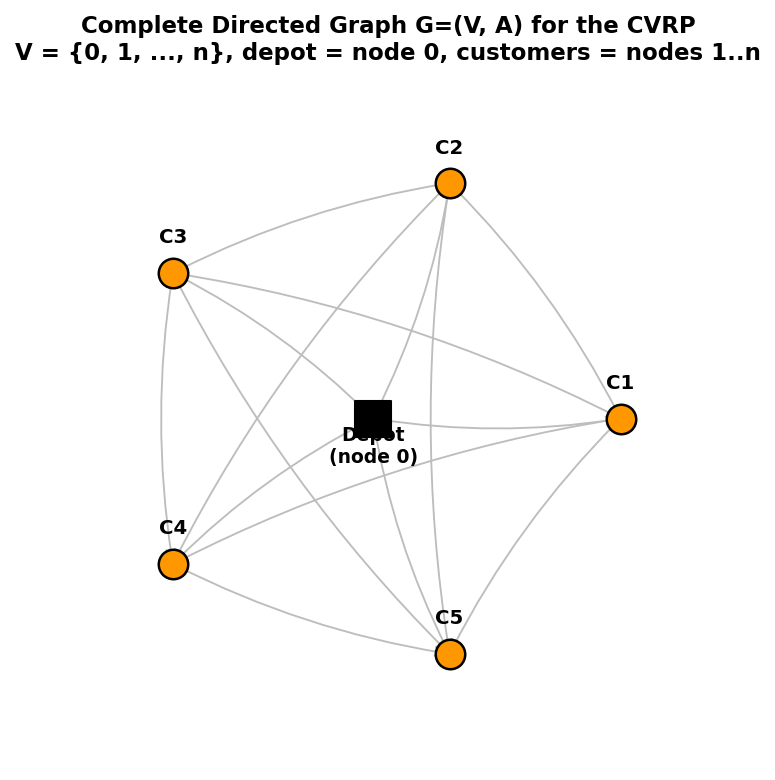
\includegraphics[width=0.65\linewidth]{cvrp_graph.png}
\end{center}

The figure above shows the complete directed graph for a small instance with 5 customers.
Every pair of nodes is connected by arcs in both directions.  In practice, because travel
costs often satisfy symmetry ($c_{ij} = c_{ji}$) and the triangle inequality, the graph
can be treated as undirected.

\medskip
\textbf{A vehicle route} is a sequence of nodes starting and ending at the depot:
\[
  r = (0, i_1, i_2, \ldots, i_k, 0)
\]
where $i_1, i_2, \ldots, i_k$ are the customers visited.
The \emph{load} of a route is $\sum_{\ell=1}^{k} d_{i_\ell}$,
and a route is \emph{feasible} if its load does not exceed $Q$.

\begin{exampleblock}{Worked Example: CVRP with 6 Customers}
Consider 6 customers with demands $d_1=3, d_2=4, d_3=3, d_4=4, d_5=3, d_6=3$
and vehicle capacity $Q=10$.
\begin{itemize}
  \item Route 1: $0 \to 1 \to 2 \to 3 \to 0$,\quad load $= 3+4+3 = 10 \leq Q$.
  \item Route 2: $0 \to 4 \to 5 \to 6 \to 0$,\quad load $= 4+3+3 = 10 \leq Q$.
\end{itemize}
Both routes are feasible.  The total cost equals the sum of all six arc distances
(e.g., $c_{01} + c_{12} + c_{23} + c_{30} + c_{04} + c_{45} + c_{56} + c_{60}$).
\end{exampleblock}

\end{frame}

\begin{frame}[allowframebreaks]{1.2.2 Mathematical Formulation (VRP-Flow Models)}

The CVRP can be formulated as an integer linear programme.  We present two
well-known formulations.

\medskip
\textbf{Sets and parameters:}
\begin{itemize}
  \item $V = \{0, 1, \ldots, n\}$: all nodes ($0$ = depot, $1\ldots n$ = customers).
  \item $V' = \{1, \ldots, n\}$: customer nodes only (the prime notation means
        ``without the depot'').
  \item $A$: set of all directed arcs $(i,j)$ with $i \neq j$.
  \item $c_{ij}$: travel cost of arc $(i,j)$.  In Euclidean instances,
        $c_{ij} = \sqrt{(x_i - x_j)^2 + (y_i - y_j)^2}$.
  \item $d_i$: demand of customer $i$ (in units compatible with $Q$; for the depot, $d_0 = 0$).
  \item $Q$: vehicle capacity (maximum load any single vehicle may carry).
  \item $K$: number of available vehicles (or, in a free-fleet formulation, a
        sufficiently large upper bound).
\end{itemize}

\textbf{Decision variables:}
\begin{itemize}
  \item $x_{ij} \in \{0, 1\}$: equals $1$ if some vehicle travels directly from
        node $i$ to node $j$, and $0$ otherwise.
        The subscript ``$ij$'' (pronounced ``$x$ sub $i$ $j$'') identifies the
        directed arc from $i$ to $j$.
  \item $u_i \geq 0$: an auxiliary integer variable for the Miller--Tucker--Zemlin
        (MTZ) subtour-elimination formulation (explained below).
\end{itemize}

\framebreak

\begin{block}{VRP-Flow Formulation (MTZ-style)}
\begin{align}
  \text{(VRP)} \quad & \min \sum_{i \in V} \sum_{j \in V,\, j \neq i} c_{ij}\, x_{ij}
  \tag{1.1} \label{eq:obj}\\[4pt]
  & \sum_{j \in V,\, j \neq i} x_{ij} = 1, \quad \forall i \in V'
  \tag{1.2} \label{eq:out}\\[4pt]
  & \sum_{i \in V,\, i \neq j} x_{ij} = 1, \quad \forall j \in V'
  \tag{1.3} \label{eq:in}\\[4pt]
  & \sum_{j \in V'} x_{0j} = K
  \tag{1.4} \label{eq:depart}\\[4pt]
  & \sum_{i \in V'} x_{i0} = K
  \tag{1.5} \label{eq:return}\\[4pt]
  & u_i - u_j + Q\, x_{ij} \leq Q - d_j, \quad \forall i \in V', j \in V', i \neq j
  \tag{1.6} \label{eq:mtz}\\[4pt]
  & d_i \leq u_i \leq Q, \quad \forall i \in V'
  \tag{1.7} \label{eq:bounds}\\[4pt]
  & x_{ij} \in \{0, 1\}, \quad \forall (i,j) \in A
  \tag{1.8} \label{eq:binary}
\end{align}
\end{block}

\framebreak

\textbf{Explanation of each constraint:}

\textbf{Objective \eqref{eq:obj}.}
The double sum $\sum_i \sum_j c_{ij} x_{ij}$ (sigma-sigma, read ``sum over all $i$
and all $j \neq i$'') accumulates the travel cost of every arc that is actually used
(i.e., where $x_{ij} = 1$).  Minimising this objective means we want the fleet to
drive as little total distance as possible.

\textbf{Constraint \eqref{eq:out}: each customer is left exactly once.}
For every customer $i$, the number of arcs leaving $i$ (i.e., arcs $(i,j)$ with
$x_{ij}=1$) equals exactly 1.  This ensures every customer is visited exactly once.

\textbf{Constraint \eqref{eq:in}: each customer is entered exactly once.}
Symmetrically, for every customer $j$, exactly one arc arrives at $j$.

\textbf{Constraints \eqref{eq:depart} and \eqref{eq:return}: fleet size.}
Exactly $K$ arcs leave the depot (one per vehicle departing) and exactly $K$ arcs
return to the depot.

\textbf{Constraint \eqref{eq:mtz}: Miller--Tucker--Zemlin subtour elimination and capacity.}
The variable $u_i$ can be interpreted as the \emph{cumulative load delivered up to
node $i$}.  If vehicle travels from $i$ to $j$ (i.e., $x_{ij}=1$), then
$u_j \geq u_i + d_j$, ensuring the cumulative load increases by $d_j$.  This
simultaneously prevents subtours (isolated cycles disconnected from the depot) and
enforces the capacity constraint.

\textbf{Constraint \eqref{eq:bounds}: load bounds.}
The cumulative load at any customer $i$ is at least $d_i$ (we have delivered at least
$i$'s own demand) and at most $Q$ (we never exceed vehicle capacity).

\begin{alertblock}{How to Read the Objective Function}
The objective says: ``add up $c_{ij}$ (the travel cost of arc $i \to j$) for every
arc that is actually used ($x_{ij}=1$), and make this total as small as possible.''
Increasing the number of vehicles generally reduces individual route lengths but may
increase total distance --- so the formula implicitly balances \emph{route efficiency}
with the number of routes.
\end{alertblock}

\framebreak

\begin{center}
  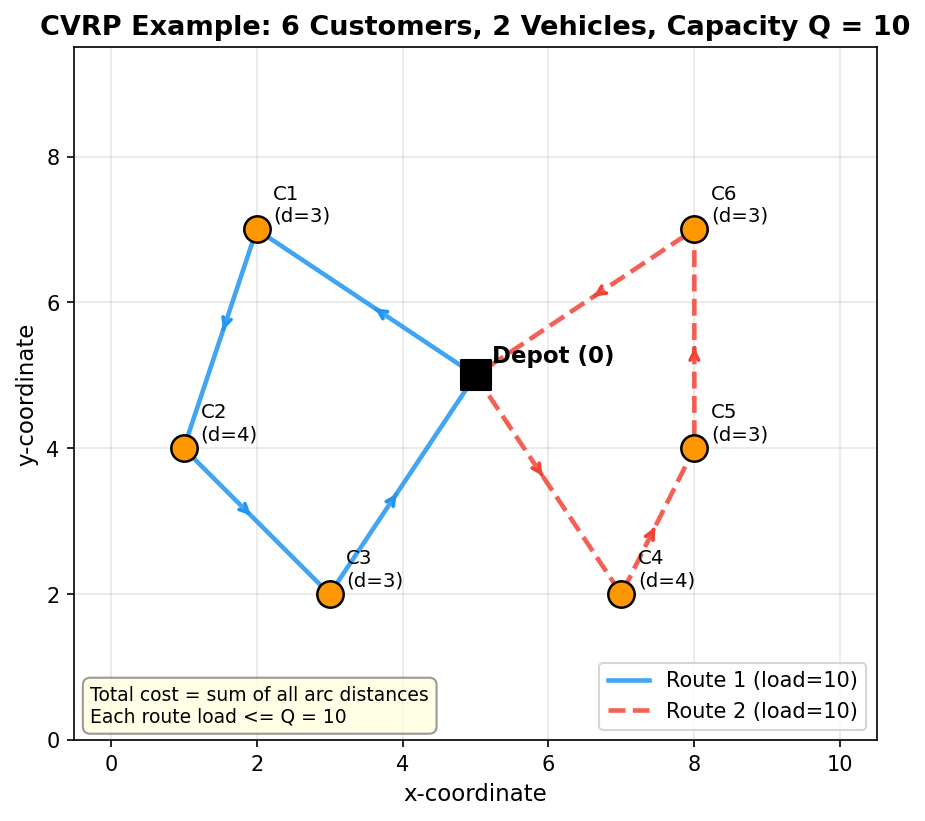
\includegraphics[width=0.62\linewidth]{cvrp_example.png}
\end{center}

This figure illustrates the CVRP with 6 customers ($n=6$) and $K=2$ vehicles of
capacity $Q=10$.  The blue (solid) route serves customers 1, 2, 3 with total load 10;
the red (dashed) route serves customers 4, 5, 6 with total load 10.  Both routes start
and end at the black square (depot, node 0).

\end{frame}

\begin{frame}[allowframebreaks]{1.2.2 Compact Formulation (Two-Index Vehicle-Flow)}

A more compact formulation uses only the binary variables $x_{ij}$.  It requires a
stronger subtour elimination mechanism, typically based on \emph{capacity inequalities}
(Laporte and Nobert 1987; Toth and Vigo 2002):

\begin{block}{Two-Index Vehicle-Flow Formulation}
\begin{align}
  \text{(VRP)} \quad & \min \sum_{(i,j)\in A} c_{ij}\, x_{ij}
  \tag{1.1$'$}\\[4pt]
  & \sum_{j \in V} x_{ij} = 1, \quad \forall i \in V'
  \tag{1.2$'$}\\[4pt]
  & \sum_{i \in V} x_{ij} = 1, \quad \forall j \in V'
  \tag{1.3$'$}\\[4pt]
  & \sum_{i \in S,\, j \notin S} x_{ij} \geq r(S), \quad \forall S \subseteq V',\ S \neq \emptyset
  \tag{Capacity cut}\\[4pt]
  & x_{ij} \in \{0, 1\}, \quad \forall (i,j)\in A
  \tag{1.8$'$}
\end{align}
\end{block}

The \textbf{capacity cut constraint} says: for any non-empty subset $S$ of customers,
the number of arcs leaving $S$ towards nodes outside $S$ must be at least $r(S)$.
Here $r(S)$ is the \emph{minimum number of vehicles needed to serve all customers in
$S$}, computed as:
\[
  r(S) = \left\lceil \frac{\sum_{i \in S} d_i}{Q} \right\rceil
\]
where $\lceil \cdot \rceil$ (ceiling function) rounds up to the nearest integer.

\framebreak

\textbf{Why do we need subtour elimination?}

Without subtour elimination, the constraints (1.2$'$) and (1.3$'$) alone only
guarantee that each customer is entered and exited exactly once --- but they do
\emph{not} prevent solutions where customers form isolated loops disconnected from
the depot.  For example, customers $\{3, 4\}$ might form a self-contained cycle
$3 \to 4 \to 3$ that never touches the depot.  Such a ``solution'' is infeasible for
routing but satisfies the in/out-degree constraints.

\begin{center}
  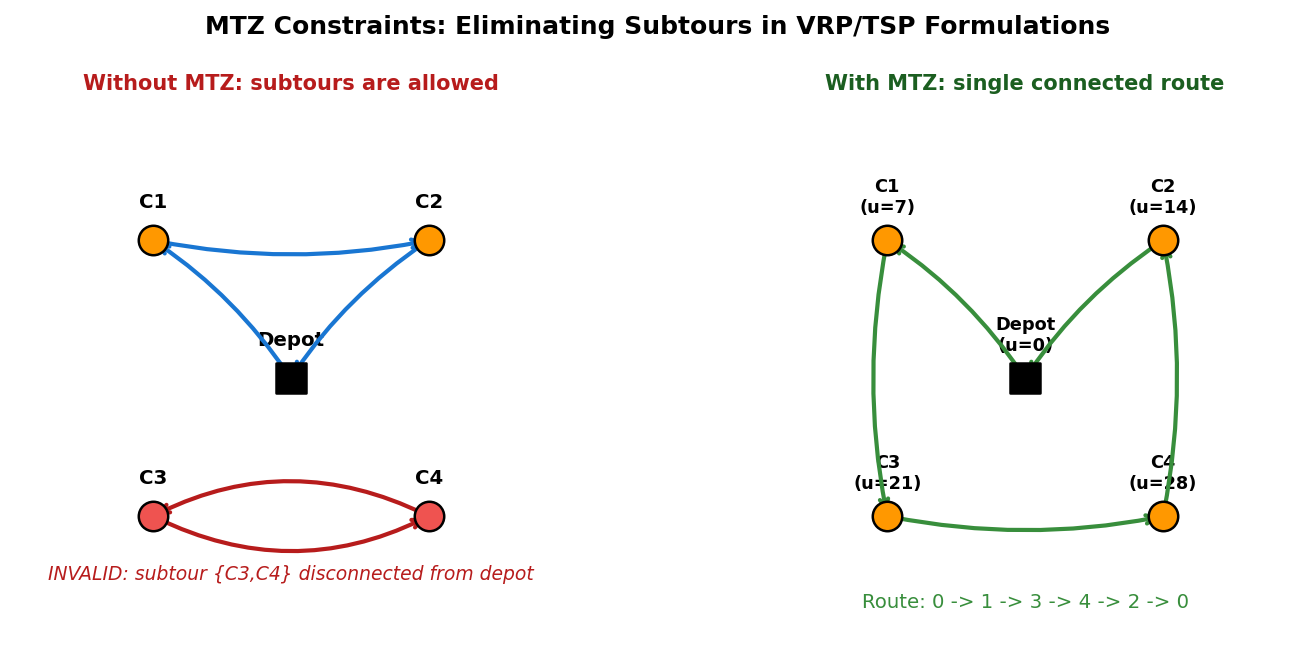
\includegraphics[width=0.58\linewidth]{mtz_subtour.png}
\end{center}

The left panel shows an invalid solution containing a subtour $\{C_3, C_4\}$
disconnected from the depot.  The right panel shows a valid single-route solution
enforced by the MTZ auxiliary variables $u_i$.

\framebreak

\begin{exampleblock}{Worked Example: MTZ Variables}
Consider 4 customers with demands $d_1=3, d_2=4, d_3=3, d_4=4$ and capacity $Q=10$.
A feasible route is $0 \to 1 \to 2 \to 3 \to 4 \to 0$, with cumulative loads:
\[
  u_1 = 3,\quad u_2 = 7,\quad u_3 = 10,\quad u_4 = 14.
\]
But $u_4 = 14 > Q = 10$, so this route \emph{violates} the capacity constraint.
The MTZ constraint (1.6) catches this: for arc $(3,4)$, we need
$u_3 - u_4 + Q \cdot x_{34} \leq Q - d_4$,
i.e., $10 - 14 + 10 \cdot 1 = 6 \leq 10 - 4 = 6$.  Equality holds, so the
constraint is satisfied --- but only because $u_3$ and $u_4$ encode the actual load.
If we tried to pretend $u_3 = 3$ and $u_4 = 3$ in a subtour, the constraint would
be violated, correctly flagging the subtour as infeasible.
\end{exampleblock}

\begin{alertblock}{Complexity Note}
The CVRP is NP-hard (it generalises the Travelling Salesman Problem, which is itself
NP-hard).  The capacity-cut formulation has an \emph{exponential} number of subtour
elimination constraints (one for each non-empty subset $S \subseteq V'$), but in
practice they are added \emph{lazily} via a branch-and-cut algorithm --- only
violated constraints are generated.
\end{alertblock}

\end{frame}

\begin{frame}[allowframebreaks]{1.2.3 Extensive Formulation (Set Partitioning)}

An alternative, elegant formulation --- the \textbf{Extensive Formulation} or
\emph{Set Partitioning} model --- was first proposed by Balinski and Quandt (1964)
and later used by Gilmore and Gomory (1965) as a starting point for column-generation
approaches.

The key idea is to \emph{enumerate all feasible routes} and then select the best
combination that covers every customer exactly once.

\medskip
\textbf{Notation:}
\begin{itemize}
  \item Let $\Omega$ (omega, pronounced ``oh-may-gah'') be the set of all feasible routes
        (each route is a sequence of customers starting and ending at the depot, with
        total load $\leq Q$).
  \item For each route $r \in \Omega$, let $c_r$ be its total travel cost.
  \item For each route $r \in \Omega$ and customer $i$, let $a_{ir} \in \{0, 1\}$ be
        an indicator: $a_{ir} = 1$ if customer $i$ is visited on route $r$, and
        $0$ otherwise.
  \item Decision variable: $\lambda_r$ (lambda, pronounced ``lam-dah'') $\in \{0, 1\}$
        equals $1$ if route $r$ is selected.
\end{itemize}

\begin{block}{Set-Partitioning Formulation (SP)}
\begin{align}
  \text{(SP)}\quad & \min \sum_{r \in \Omega} c_r\, \lambda_r
  \tag{1.9}\\[4pt]
  & \sum_{r \in \Omega} a_{ir}\, \lambda_r = 1, \quad \forall i \in V'
  \tag{1.10}\\[4pt]
  & \sum_{r \in \Omega} \lambda_r \leq K
  \tag{1.11}\\[4pt]
  & \lambda_r \in \{0, 1\}, \quad \forall r \in \Omega
  \tag{1.12}
\end{align}
\end{block}

\framebreak

\textbf{Explanation:}

\textbf{Objective (1.9).} Minimise the total cost of all selected routes.

\textbf{Constraint (1.10): coverage.}
For each customer $i$, the sum of $a_{ir} \lambda_r$ over all routes $r$ must equal
exactly 1.  In plain words: customer $i$ must appear in exactly one selected route.
(This is the ``partition'' in set partitioning --- customers are partitioned among routes.)

\textbf{Constraint (1.11): fleet size.}
At most $K$ routes are selected (at most $K$ vehicles depart).

\begin{alertblock}{Why This Formulation?}
The SP formulation is very clean and its LP relaxation provides extremely tight lower
bounds.  Modern exact VRP solvers are almost always based on column generation applied
to the LP relaxation of the SP formulation, combined with branch-and-bound.  The
column generation subproblem --- finding the route $r$ with the most negative reduced
cost --- is a constrained shortest-path problem, itself NP-hard but solvable with
dynamic programming via labelling algorithms.
\end{alertblock}

\textbf{Practical limitation:} The set $\Omega$ of all feasible routes can be
astronomically large --- exponential in $n$.  Therefore the SP model cannot be solved
directly by enumerating all columns.  Instead, \emph{column generation} dynamically
adds only the most promising routes during LP solving.

\end{frame}

% ============================================================
\section{1.3 The Family of VRP}
% ============================================================

\begin{frame}[allowframebreaks]{Overview of the VRP Family}

Over decades of research, the basic CVRP has been extended in many directions to
capture additional real-world constraints and objectives.  The resulting collection
of variants is referred to as \textbf{the family of vehicle routing problems}.

\begin{center}
  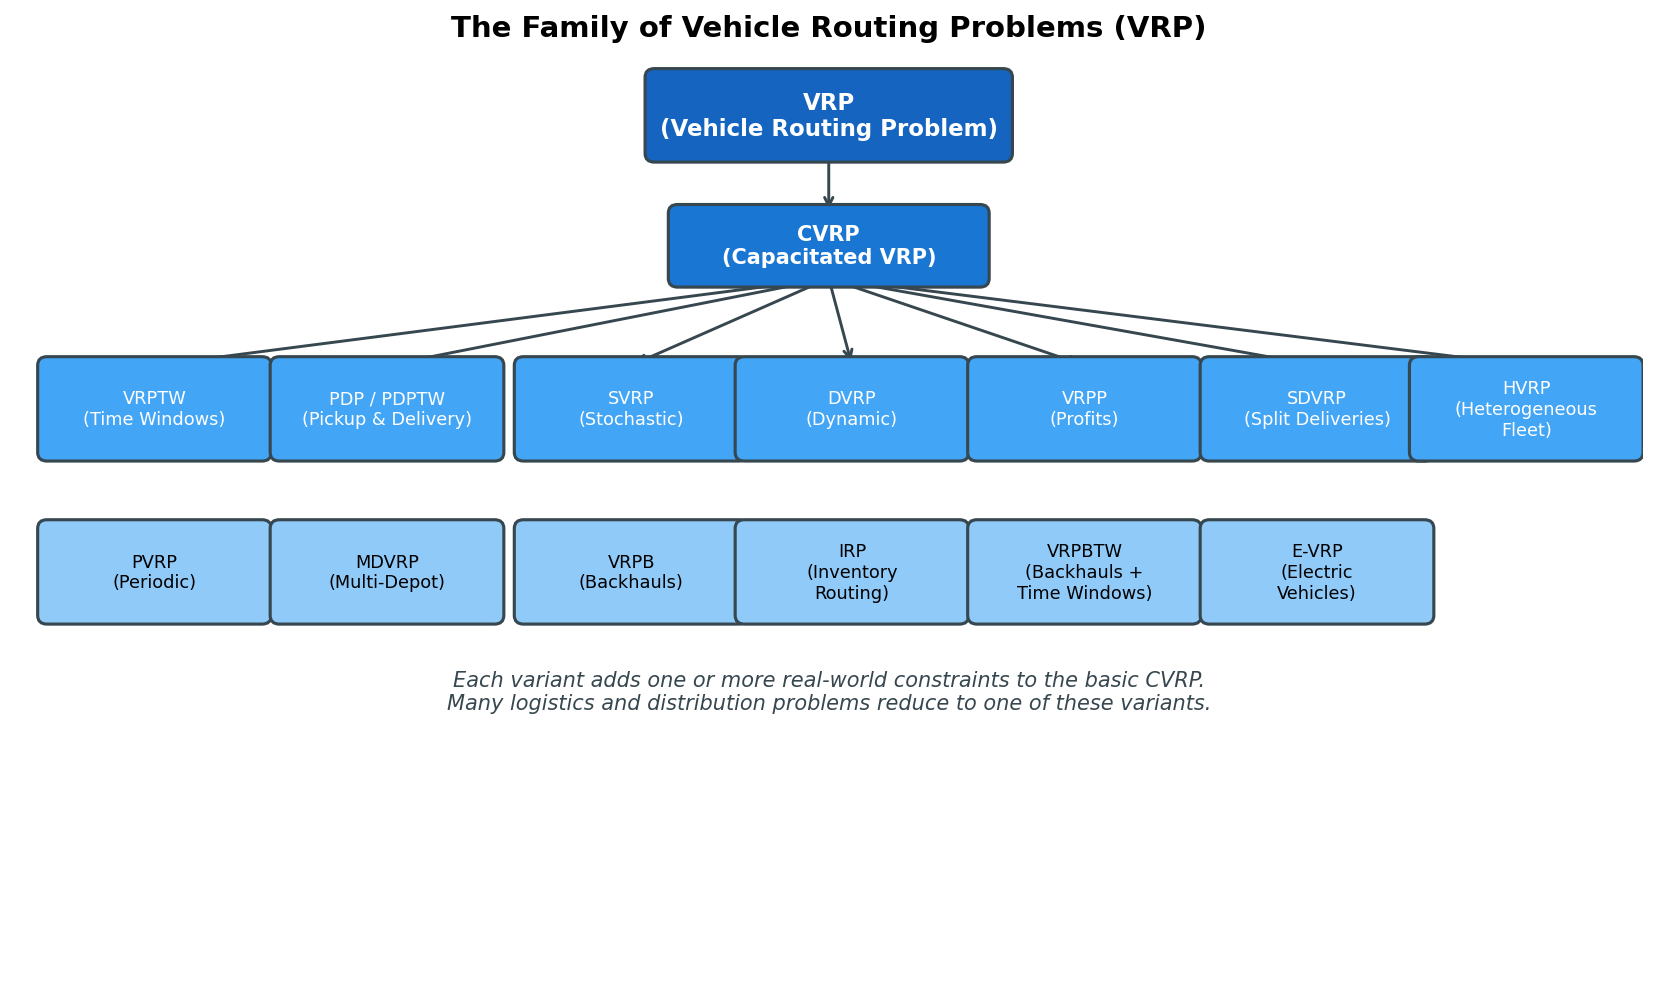
\includegraphics[width=0.88\linewidth]{vrp_taxonomy.png}
\end{center}

The figure above shows the taxonomy of major VRP variants.  Each box adds one or more
constraints (or relaxations) to the basic CVRP.  Variants can also be combined ---
for example, a VRPTW with heterogeneous fleet, or a stochastic PDPTW.

\end{frame}

\begin{frame}[allowframebreaks]{1.3.1 Network and Customer Characteristics}

Before discussing specific variants, it is useful to understand the \emph{building
blocks} that differentiate VRP variants.  The first building block concerns the
characteristics of the underlying network and the customers.

\medskip
\textbf{Transportation requests.}
In the basic CVRP, each customer $i$ has a single demand $d_i$ that must be
\emph{delivered} from the depot.  More general settings include:

\begin{itemize}
  \item \textbf{Delivery and Collection:} some customers receive goods (delivery, also
        called \emph{linehaul}) while others send goods back to the depot (collection,
        also called \emph{backhaul}).  The \emph{VRP with Backhauls (VRPB)} requires
        all deliveries on a route to be completed before any pickups begin.

  \item \textbf{Pickup and Delivery:} goods are transported between pairs of locations
        $(p_i, d_i)$ --- picked up at $p_i$ and delivered to $d_i$.  The vehicle must
        visit $p_i$ before $d_i$ on the same route.  This is the
        \emph{Pickup and Delivery Problem (PDP)}.

  \item \textbf{Non-split Deliveries:} each customer's demand must be served by a single
        vehicle in a single visit.  This is the standard CVRP assumption.

  \item \textbf{Split Deliveries:} a customer's demand may be split across multiple
        vehicles.  This can reduce total distance but requires coordination.
\end{itemize}

\framebreak

\textbf{Loading constraints.}
The vehicle is not just a container with a scalar capacity.  Real vehicles have a
3-dimensional interior, and the order in which goods are loaded matters:
\begin{itemize}
  \item \emph{Last-In-First-Out (LIFO):} if goods are stacked, the last item loaded
        must be the first unloaded.  This imposes a constraint on the order of
        deliveries within a route.
  \item \emph{2D/3D bin packing:} goods must physically fit in the vehicle's cargo space.
        This couples the routing problem with a bin packing problem.
\end{itemize}

\textbf{Multiple depots.}
In the \emph{Multi-Depot VRP (MDVRP)}, there are several depots.  Vehicles can start
and end at different depots, and customers must be assigned to depots.

\textbf{Alternative delivery locations.}
A customer can be served at one of several alternative locations (e.g., collection
points, lockers).  This relaxes the geographical constraint and can reduce total
distance.

\end{frame}

\begin{frame}[allowframebreaks]{1.3.2 Time Windows (VRPTW)}

The \textbf{Vehicle Routing Problem with Time Windows (VRPTW)} is probably the most
widely studied VRP variant.  It extends the CVRP by associating a \emph{time window}
$[a_i, b_i]$ with each customer $i$ and with the depot.

\begin{block}{Time Window Constraint}
A vehicle must arrive at customer $i$ no earlier than $a_i$ (\emph{earliest service
time}) and no later than $b_i$ (\emph{latest service time}).  If it arrives before
$a_i$, it must \emph{wait} until $a_i$ to begin service.  If it cannot arrive by
$b_i$, the solution is \emph{infeasible}.
\end{block}

\textbf{Additional notation for VRPTW:}
\begin{itemize}
  \item $s_i$: service time at customer $i$ (time spent unloading goods).
  \item $t_{ij}$: travel time on arc $(i,j)$ (may differ from cost $c_{ij}$).
  \item $w_i \geq 0$: waiting time at customer $i$ (non-negative; vehicle must wait
        if it arrives early).
  \item $T_i$: time at which service \emph{begins} at customer $i$.
\end{itemize}

The service-start time propagates along a route:
\[
  T_j = \max\bigl(a_j,\; T_i + s_i + t_{ij}\bigr)
\]
This says: service at $j$ begins either at the earliest allowed time $a_j$, or as
soon as the vehicle arrives (after completing service at $i$, travelling to $j$),
whichever is later.  The $\max$ function captures the \emph{waiting} behaviour.

\framebreak

\begin{center}
  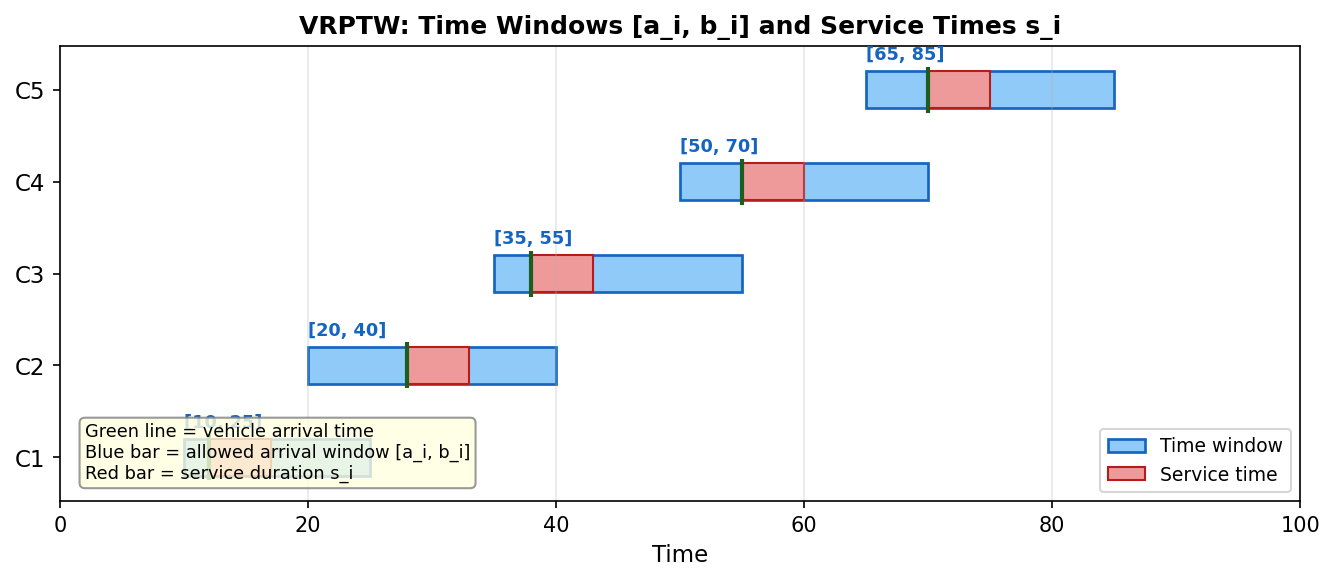
\includegraphics[width=0.72\linewidth]{vrptw_time_windows.png}
\end{center}

The figure shows time windows $[a_i, b_i]$ (blue bars) for five customers.  The green
vertical line marks the vehicle's arrival time at each customer.  The red bar shows
service duration $s_i$.

\medskip
\textbf{Types of time windows:}
\begin{itemize}
  \item \emph{Hard time windows:} violation of $b_i$ makes the solution infeasible.
        This is the standard VRPTW constraint.
  \item \emph{Soft time windows:} arriving after $b_i$ is allowed but incurs a
        penalty cost proportional to the delay.  This is a common practical
        extension (e.g., penalise late deliveries by \$10 per minute).
\end{itemize}

\begin{alertblock}{Key Insight: Why Time Windows Are Hard}
Time windows create \emph{cascading dependencies} among the customers on a route ---
a delay at one customer propagates and may push arrival at every subsequent customer
outside its window.  This makes the VRPTW significantly harder than the CVRP.
Benchmark instances from Solomon (1987) remain standard for evaluating algorithms.
\end{alertblock}

\framebreak

\textbf{VRPTW Formulation variables (extending CVRP):}
\begin{itemize}
  \item $x_{ij} \in \{0,1\}$: arc usage (same as CVRP).
  \item $T_i \geq 0$: service start time at customer $i$.
\end{itemize}

The additional constraints for the VRPTW are:
\begin{align*}
  T_i + s_i + t_{ij} - M(1 - x_{ij}) &\leq T_j,
  \quad \forall i \in V,\, j \in V', i \neq j\\
  a_i &\leq T_i \leq b_i, \quad \forall i \in V
\end{align*}
where $M$ (capital M) is a sufficiently large constant (a \emph{big-M} coefficient).
The first constraint says: if the vehicle uses arc $(i,j)$ (i.e., $x_{ij}=1$), then
$T_j \geq T_i + s_i + t_{ij}$ --- time at $j$ is at least time at $i$ plus service
time plus travel time.  When $x_{ij}=0$, the constraint is rendered inactive by the
$-M$ term.

\end{frame}

\begin{frame}[allowframebreaks]{1.3.3 Pickup and Delivery (PDP / PDPTW)}

In the basic CVRP, goods flow \emph{from the depot to customers}.  The
\textbf{Pickup and Delivery Problem (PDP)} generalises this by allowing goods to
flow between any pair of locations in the network.

\begin{block}{Pickup and Delivery Problem (PDP)}
Each transportation request $r = (p_r, d_r, q_r)$ consists of:
\begin{itemize}
  \item $p_r$: pickup location (the origin --- where goods are collected).
  \item $d_r$: delivery location (the destination --- where goods are dropped off).
  \item $q_r$: quantity of goods (demand for this request).
\end{itemize}
A vehicle that handles request $r$ must visit $p_r$ \emph{before} $d_r$ on the same
route, and must carry the goods from $p_r$ to $d_r$ without exceeding capacity.
\end{block}

\begin{center}
  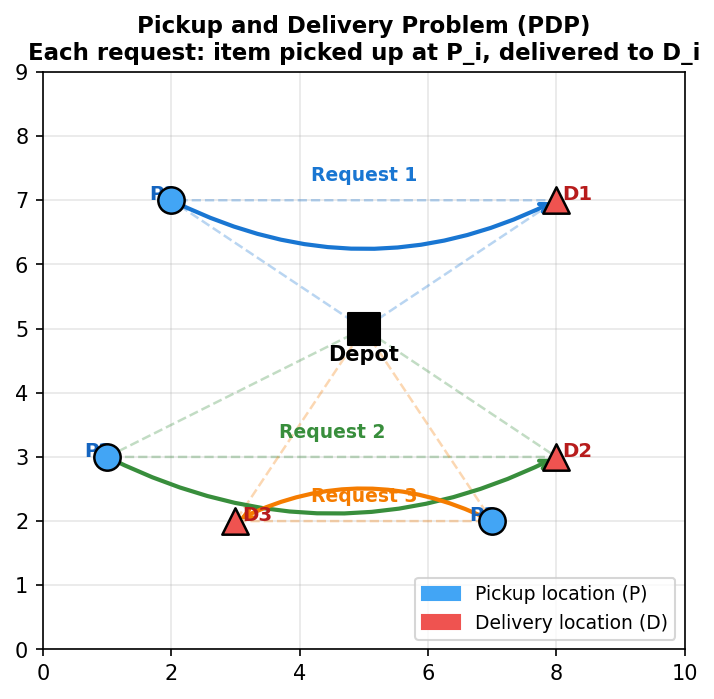
\includegraphics[width=0.55\linewidth]{pickup_delivery.png}
\end{center}

\framebreak

\textbf{Variants of the PDP:}

\begin{itemize}
  \item \textbf{One-to-one PDP (1-1 PDP):} Each request has one specific origin and
        one specific destination.  This is the most general form.  Applications:
        courier services, taxi/ridesharing, mail delivery.

  \item \textbf{Many-to-one PDP (collection):} Multiple origins, one destination
        (the depot).  Example: collecting goods from suppliers and bringing them to
        a warehouse.

  \item \textbf{One-to-many PDP (distribution):} One origin (depot), multiple
        destinations.  This reduces to the standard CVRP.

  \item \textbf{PDPTW:} PDP with time windows at both pickup and delivery locations.
        This is the most constrained and most studied variant.
\end{itemize}

\begin{alertblock}{Key Precedence Constraint}
The constraint that the pickup $p_r$ must be visited \emph{before} the delivery
$d_r$ on the same route is a \emph{precedence constraint}.  It fundamentally
changes the structure of feasible solutions compared to the CVRP and makes the
PDPTW significantly harder.
\end{alertblock}

\end{frame}

\begin{frame}[allowframebreaks]{1.3.4 Stochastic VRP (SVRP)}

In practice, some input data --- customer demands, travel times, or even which
customers will request service --- may not be known precisely in advance.  The
\textbf{Stochastic VRP (SVRP)} models this uncertainty explicitly.

\begin{block}{Three Main Sources of Stochasticity}
\begin{enumerate}
  \item \textbf{Stochastic demands:} Customer $i$ has a random demand
        $D_i$ (capital $D$ to denote a random variable) drawn from a known probability
        distribution.  The mean and variance of $D_i$ are known at planning time,
        but the actual value is revealed only when the vehicle arrives at $i$.
  \item \textbf{Stochastic travel times:} Travel time on arc $(i,j)$ is a random
        variable, modelling traffic congestion or weather effects.
  \item \textbf{Stochastic customers:} Not all customers in the potential set will
        actually request service.  Customer $i$ is present with probability $p_i$
        (p sub i).
\end{enumerate}
\end{block}

\begin{center}
  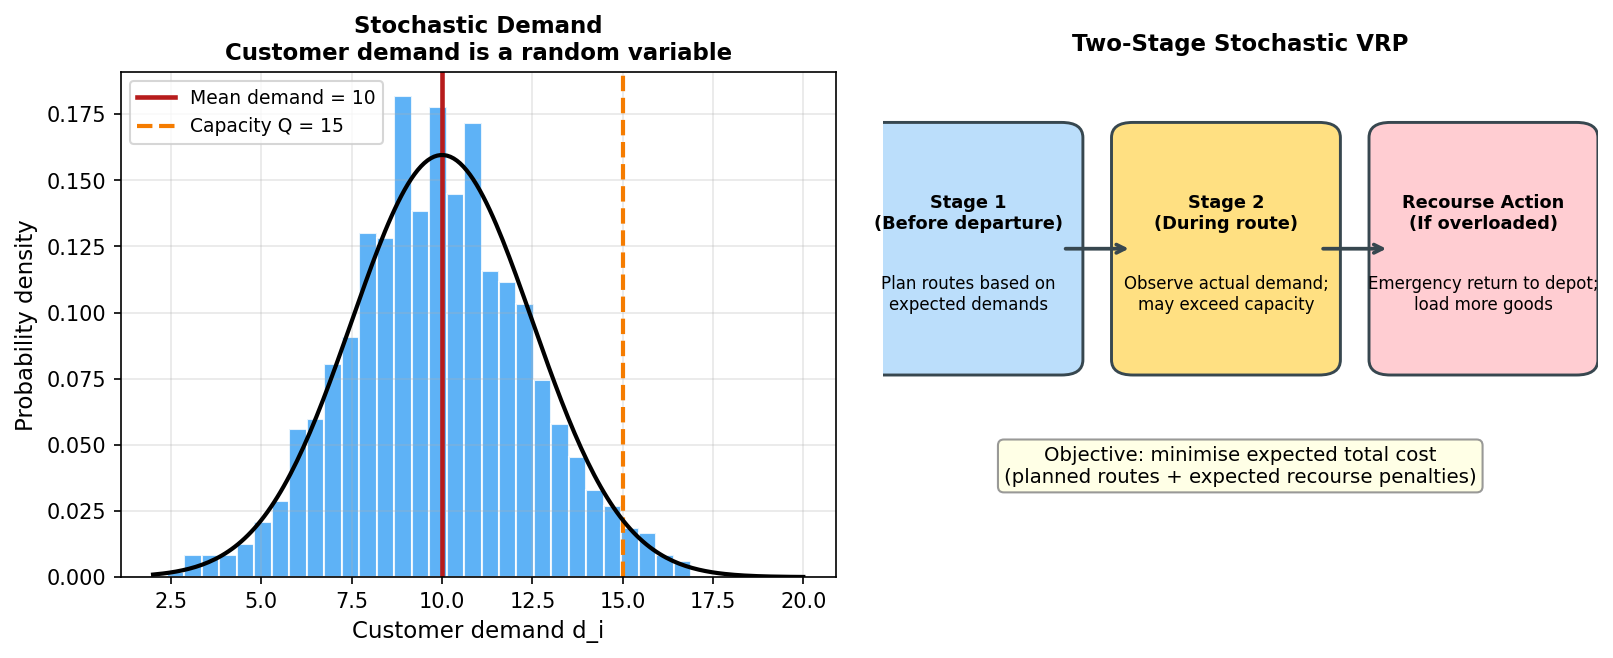
\includegraphics[width=0.72\linewidth]{stochastic_vrp.png}
\end{center}

\framebreak

\textbf{Two-Stage Stochastic Programming Framework:}

The SVRP is naturally modelled as a \emph{two-stage stochastic programme}:

\begin{itemize}
  \item \textbf{Stage 1 (here-and-now):} Before any uncertainty is revealed, plan
        routes based on expected/known data.  These are the \emph{first-stage} decisions.
  \item \textbf{Stage 2 (wait-and-see / recourse):} Once uncertainty is revealed
        during route execution, take \emph{recourse actions} to restore feasibility.
\end{itemize}

The most common recourse action for the SVRP with stochastic demands is the
\emph{vehicle return to depot}: if a vehicle arrives at customer $i$ and finds that
its remaining capacity is insufficient to serve $i$'s actual demand, it returns to
the depot to reload, then comes back to $i$.

\begin{block}{Objective Function of the SVRP}
\[
  \min\; c(\text{first-stage route}) + \mathbb{E}_{\boldsymbol{D}}\bigl[Q(\text{route}, \boldsymbol{D})\bigr]
\]
Here $\mathbb{E}$ (blackboard-bold E) denotes the \emph{expected value} (mathematical
expectation) over the random vector $\boldsymbol{D}$ (bold $D$) of all customer demands.
$Q(\text{route}, \boldsymbol{D})$ is the recourse cost (extra distance due to emergency
depot returns) given the realised demands $\boldsymbol{D}$.
\end{block}

The key challenge of the SVRP is that $\mathbb{E}[Q]$ is generally hard to compute
analytically and must be estimated by Monte Carlo simulation or approximated by
closed-form bounds.

\end{frame}

\begin{frame}[allowframebreaks]{1.3.5 Dynamic VRP (DVRP)}

The \textbf{Dynamic VRP (DVRP)} arises when information about transportation requests
becomes available \emph{during the execution of routes} --- not all requests are known
at the time of planning.

\begin{center}
  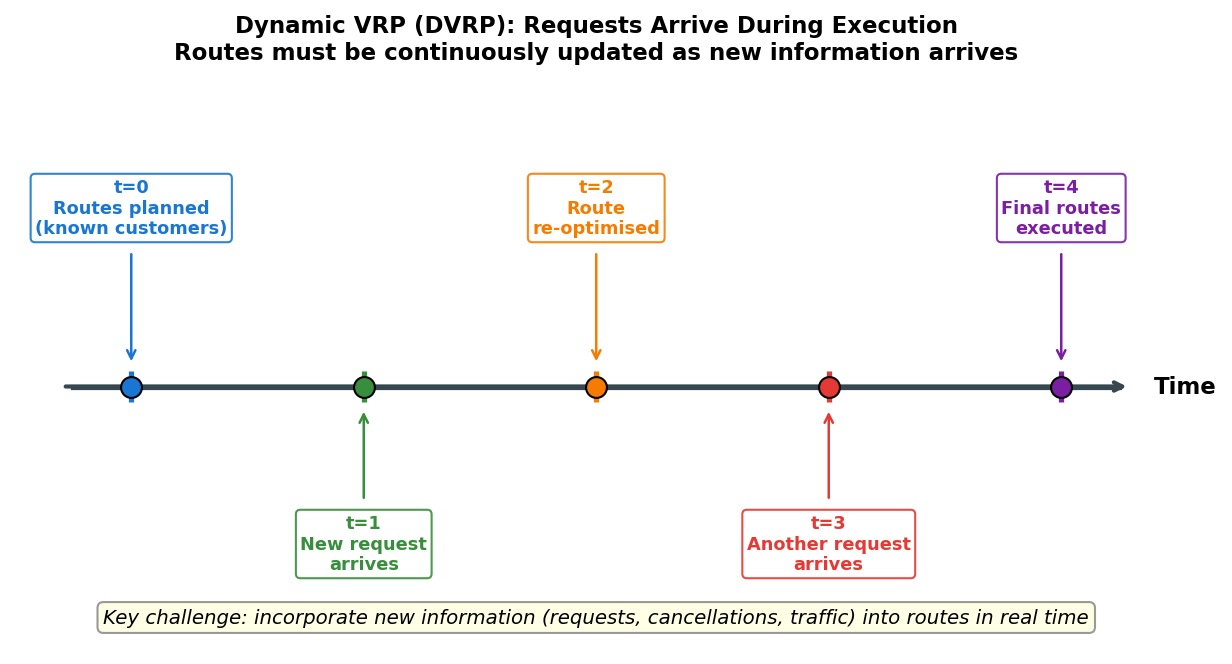
\includegraphics[width=0.72\linewidth]{dynamic_vrp.png}
\end{center}

\textbf{What makes a VRP dynamic?}
The degree of dynamism (DoD) characterises how much of the routing information is
known in advance.  Formally, if $n_d$ (n-sub-d) is the number of requests known only
during execution, and $n$ is the total number of requests, then:
\[
  \text{DoD} = \frac{n_d}{n}
\]
A DoD of 0 means the problem is fully static (all information known upfront).
A DoD of 1 means all requests arrive online with no advance information.

\framebreak

\textbf{Real-time management decisions in DVRP:}
\begin{enumerate}
  \item \textbf{Acceptance/rejection:} Decide in real time whether to accept a new
        request.
  \item \textbf{Route modification:} Insert the new request into the best position in
        an existing route, or create a new route.
  \item \textbf{Re-optimisation:} Periodically re-optimise all routes to incorporate
        accumulated new information.
\end{enumerate}

\textbf{Relationship to stochastic VRP:}
Stochastic VRPs and dynamic VRPs are related but distinct:
\begin{itemize}
  \item In the \emph{stochastic} VRP, uncertainty is modelled \emph{probabilistically}
        and taken into account at planning time.
  \item In the \emph{dynamic} VRP, new information simply \emph{arrives} during execution
        without a prior probabilistic model.
  \item A problem can be both stochastic \emph{and} dynamic (e.g., the demand at a
        newly revealed customer is itself uncertain).
\end{itemize}

\begin{alertblock}{Practical Applications}
Dynamic VRPs model taxi dispatching, ambulance routing, same-day delivery,
ride-hailing (e.g., Uber/Lyft), and emergency vehicle routing.  Real-time
algorithms must respond within seconds to each new request.
\end{alertblock}

\end{frame}

\begin{frame}[allowframebreaks]{1.3.6 VRP with Profits (VRPP)}

In the standard CVRP and VRPTW, \emph{all} customers must be served.  The
\textbf{VRP with Profits (VRPP)} relaxes this constraint: each customer $i$ has a
\emph{profit} (or prize) $\pi_i$ (pi, pronounced ``pie'') associated with visiting it,
and the planner decides which customers to visit.

\begin{block}{VRPP Objective}
Maximise the total collected profit minus the total travel cost:
\[
  \max \sum_{i \in S} \pi_i - \sum_{(i,j) \in \text{routes}} c_{ij}
\]
where $S \subseteq V'$ is the set of \emph{selected} customers (customers that are
actually visited).  The planner is free to skip any customer, but skipping customer
$i$ means forgoing profit $\pi_i$.
\end{block}

\textbf{Two main sub-variants:}

\begin{itemize}
  \item \textbf{Orienteering Problem (OP):} A single vehicle, a time limit $T_{\max}$,
        and profits $\pi_i$ at nodes.  The vehicle starts and ends at the depot.
        Maximise the total profit collected within the time budget.  This is named after
        the sport of orienteering, where a competitor collects checkpoints within a
        time limit.

  \item \textbf{Profitable Tour Problem (PTP):} Multiple vehicles; choose which
        customers to visit to maximise net profit (collected profits minus routing costs).
        No hard upper bound on number of vehicles.
\end{itemize}

\begin{alertblock}{Key Insight}
The VRPP trades off \emph{visit benefit} (profit) against \emph{visit cost} (distance).
A customer far from the route is only worth visiting if its profit $\pi_i$ exceeds the
extra distance $\delta c$ incurred by detouring to it.  The formula for the detour cost
of inserting customer $i$ between customers $j$ and $k$ is:
$\delta c = c_{ji} + c_{ik} - c_{jk}$.
\end{alertblock}

\end{frame}

\begin{frame}[allowframebreaks]{1.3.7 Split Deliveries (SDVRP)}

In the standard CVRP, each customer's full demand must be served in a single visit
by a single vehicle.  The \textbf{Split Delivery VRP (SDVRP)} relaxes this assumption.

\begin{block}{Split Delivery}
In the SDVRP, a customer $i$ with demand $d_i > Q$ (greater than vehicle capacity)
\emph{must} be served by multiple vehicles.  More generally, even when $d_i \leq Q$,
it may be \emph{beneficial} to split a customer's demand across vehicles to reduce
total routing distance.
\end{block}

\begin{center}
  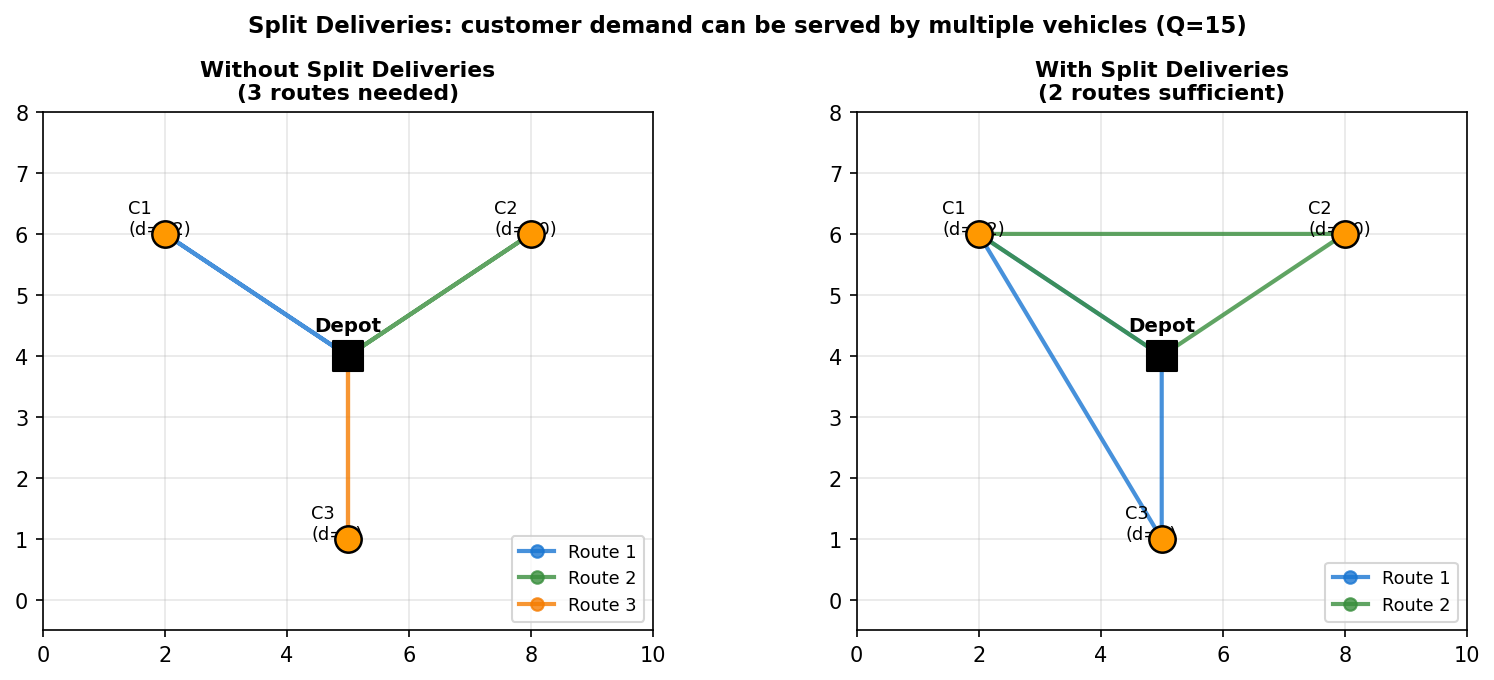
\includegraphics[width=0.72\linewidth]{split_deliveries.png}
\end{center}

\framebreak

\textbf{When does splitting help?}

Consider 3 customers with demands $d_1=12, d_2=10, d_3=8$ and vehicle capacity $Q=15$.
Without splitting, we need 3 vehicles (one per customer, since no pair fits in one
vehicle: $d_1+d_2=22>Q$, $d_1+d_3=20>Q$, $d_2+d_3=18>Q$).

With splitting:
\begin{itemize}
  \item Route 1: serve customer 1 partially (7 units) and customer 3 fully (8 units).
        Load $= 7 + 8 = 15 = Q$.
  \item Route 2: serve customer 2 fully (10 units) and remaining demand of customer 1
        (5 units).  Load $= 10 + 5 = 15 = Q$.
\end{itemize}
Only 2 vehicles needed --- a saving of one vehicle.

\begin{alertblock}{Modelling Complexity}
Split deliveries significantly increase solution space complexity because the quantity
delivered to each customer becomes a continuous decision variable, on top of the
combinatorial routing decisions.  However, they can produce substantially cheaper
solutions for large-demand customers.
\end{alertblock}

\end{frame}

\begin{frame}[allowframebreaks]{1.3.8 Heterogeneous Fleet (HVRP)}

The standard CVRP assumes all vehicles are identical (same capacity $Q$, same cost
per kilometre).  In practice, fleets are often \emph{heterogeneous}: different vehicle
types have different capacities, fixed costs, and variable travel costs.

\begin{center}
  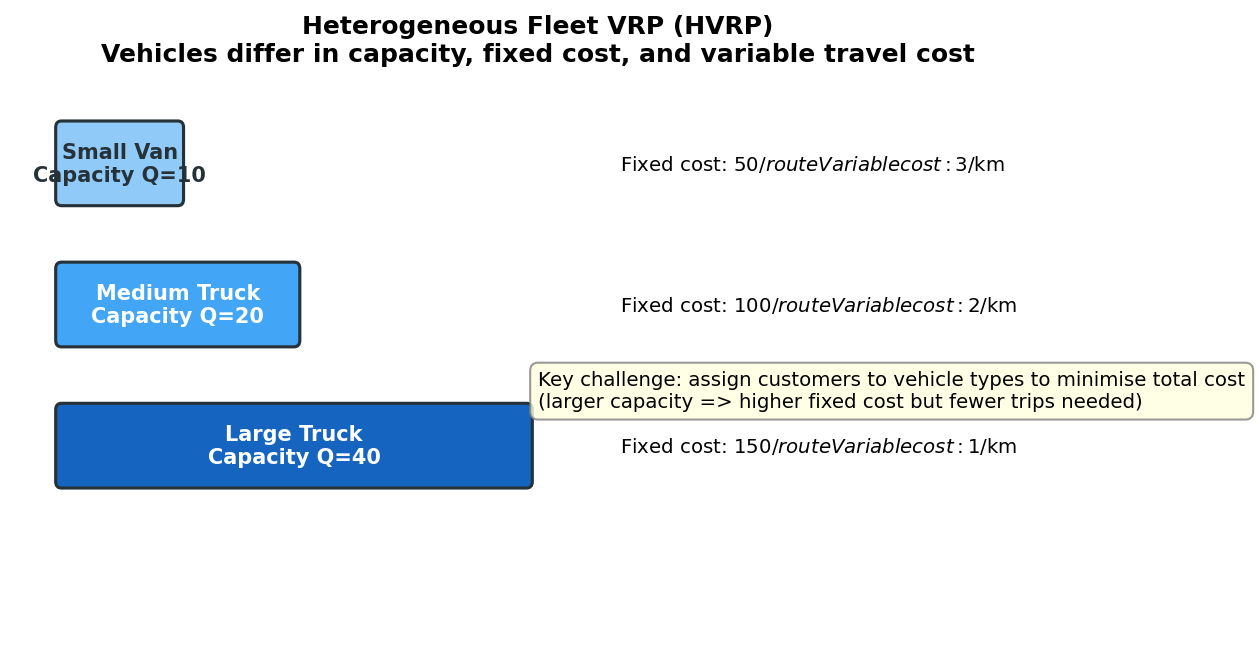
\includegraphics[width=0.65\linewidth]{heterogeneous_fleet.png}
\end{center}

\begin{block}{Heterogeneous Fleet VRP (HVRP)}
There are $T$ vehicle types.  Vehicle of type $t$ has:
\begin{itemize}
  \item capacity $Q_t$ (Q-sub-t): maximum load.
  \item fixed cost $f_t$ (f-sub-t): cost incurred whenever a vehicle of type $t$ is used,
        regardless of its route.
  \item variable cost $v_t$ (v-sub-t): cost per unit of distance travelled by a type-$t$
        vehicle.
\end{itemize}
\end{block}

\framebreak

\textbf{Two sub-variants:}
\begin{itemize}
  \item \textbf{Fleet Size and Mix VRP (FSM):} The number of available vehicles of
        each type is \emph{unlimited}.  The optimiser decides how many of each type to
        use.  This is called a ``fleet composition'' problem.
  \item \textbf{Heterogeneous VRP (HVRP):} The number of vehicles of each type is
        \emph{fixed} in advance.  The optimiser only decides which type serves which
        customers.
\end{itemize}

\textbf{Objective function for HVRP:}
\[
  \min \sum_{t=1}^{T} f_t k_t + \sum_{r \in \Omega} c_r \lambda_r
\]
where $k_t$ is the number of vehicles of type $t$ used, and $c_r$ is the cost of
route $r$ (using the appropriate variable cost for the assigned vehicle type).

\begin{alertblock}{Trade-off: Capacity vs.\ Cost}
Using a large truck reduces the number of routes needed (fewer vehicles), but incurs
a higher fixed cost.  Using many small vans avoids fixed costs but requires more
routes and therefore more total travel.  The HVRP must balance these competing
incentives.
\end{alertblock}

\end{frame}

\begin{frame}[allowframebreaks]{1.3.9 Periodic VRP (PVRP)}

The \textbf{Periodic VRP (PVRP)} extends the CVRP to a multi-day planning horizon.
Each customer must be visited a specified number of times (\emph{frequency}) over
the planning period, and the planner must decide \emph{on which days} to visit each
customer.

\begin{center}
  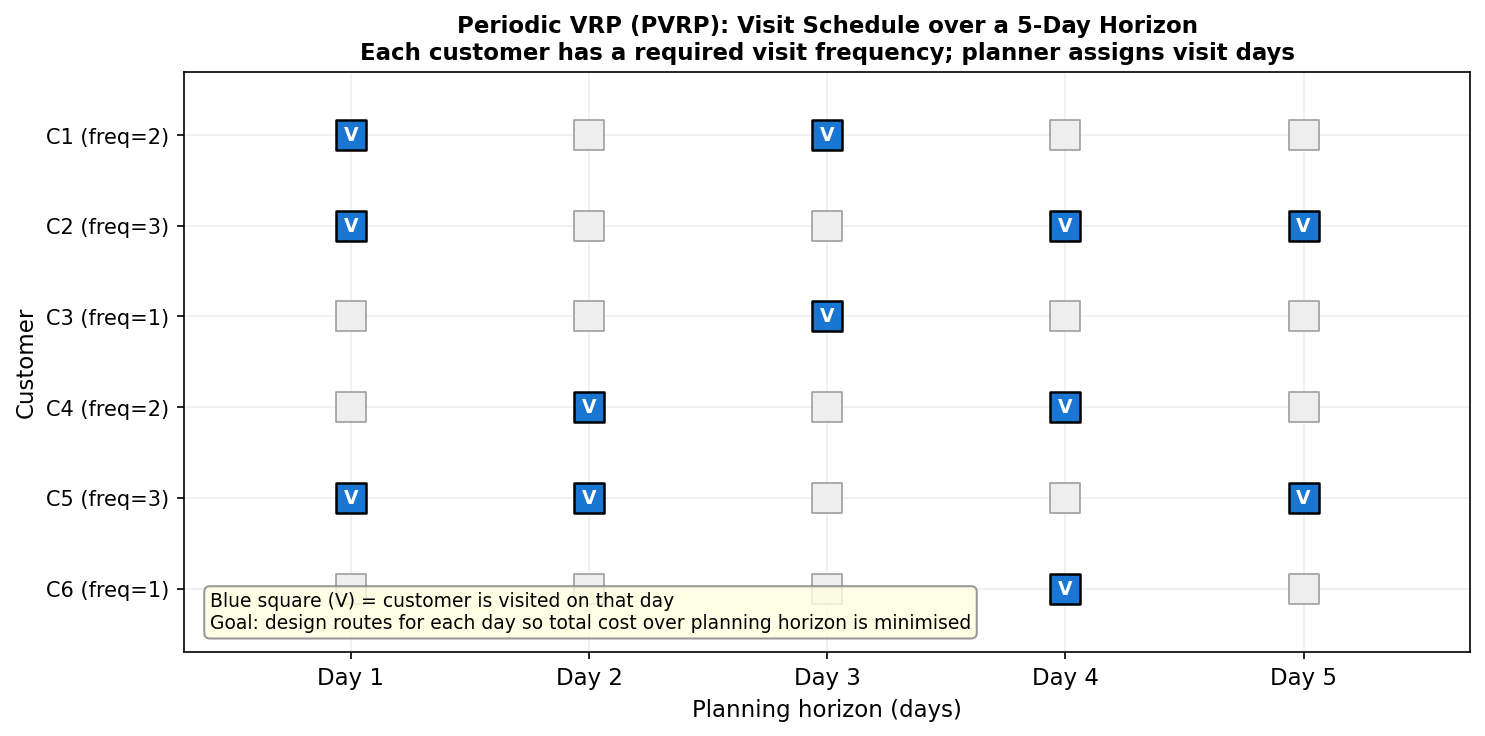
\includegraphics[width=0.72\linewidth]{periodic_vrp.png}
\end{center}

\textbf{Example:} A customer who needs deliveries 3 times per week (frequency = 3)
in a 5-day horizon can be visited on days $\{1,2,3\}$, $\{1,2,5\}$, $\{1,3,5\}$,
$\{2,3,4\}$, etc.  These are the \emph{feasible visit combinations} for this customer.

\framebreak

\begin{block}{PVRP Formulation}
Let $\mathcal{T} = \{1, 2, \ldots, T\}$ be the set of days in the planning horizon.
For each customer $i$, let $\mathcal{P}_i$ be the set of feasible visit combinations
(day-subsets of $\mathcal{T}$ with the right frequency).  A \emph{schedule} for
customer $i$ selects one combination $p \in \mathcal{P}_i$.

The PVRP must simultaneously:
\begin{enumerate}
  \item Assign each customer a visit combination (which days to visit).
  \item Design one route per day that covers all customers assigned to that day.
\end{enumerate}
The objective is to minimise the total routing cost over all days.
\end{block}

\begin{alertblock}{Why PVRP Is Harder Than CVRP}
The PVRP has an additional combinatorial dimension: the assignment of customers to
days.  This creates interdependencies across days --- choosing a poor visit schedule
for one customer can inflate routing costs on all affected days.  The PVRP is a
two-level combinatorial optimisation problem.
\end{alertblock}

\end{frame}

\begin{frame}[allowframebreaks]{1.3.10 Intra-route Constraints}

So far we have focused on \emph{inter-route} constraints (which routes to create,
how many vehicles, capacity).  But many practical problems impose additional
\emph{intra-route} constraints that restrict the \emph{ordering} of customers within
a single route.

\medskip
\textbf{Loading constraints --- Last-In-First-Out (LIFO).}
When loading a van, goods placed at the back of the vehicle are accessed last.
If the vehicle visits customers in the order $i_1, i_2, \ldots, i_k$, then goods
for customer $i_k$ must be loaded \emph{last} (closest to the door).  Formally,
the LIFO constraint requires that goods are loaded in reverse order of delivery.
This rules out many otherwise optimal routes and is known to increase routing costs
significantly.

\medskip
\textbf{First-In-First-Out (FIFO).}
In some contexts (e.g., fragile stacked goods), the loading sequence must follow the
delivery sequence.  FIFO loading constrains routes differently from LIFO.

\medskip
\textbf{Precedence constraints.}
As in the PDP, customer $j$ may only be visited \emph{after} customer $i$ on the
same route.  This can model assembly-line-style logistics or sequential operations.

\medskip
\textbf{Synchronisation constraints.}
Two vehicles may need to be at the same location at the same time (e.g., for a
vehicle transfer, or for a two-person job).  Synchronisation constraints link
the routes of different vehicles.

\end{frame}

% ============================================================
\section{1.4 Objectives}
% ============================================================

\begin{frame}[allowframebreaks]{1.4 Objectives in VRP}

The objective function is a fundamental component of any VRP formulation.  The
choice of objective reflects the economic goal of the routing planner.

\begin{block}{Single Objective: Minimise Total Distance}
The most common objective in the research literature:
\[
  \min \sum_{(i,j) \in A} c_{ij}\, x_{ij}
\]
This minimises the total distance (or equivalently, total travel cost) driven by
all vehicles.  When $c_{ij}$ represents fuel cost, this objective directly minimises
fuel expenditure.
\end{block}

\begin{block}{Minimise Number of Vehicles}
A secondary, hierarchically superior objective used in many benchmark studies:
\[
  \min K \quad \text{(number of vehicles used)}
\]
In a lexicographic (two-level) objective, first minimise $K$, then minimise total
distance.  This reflects the reality that reducing fleet size frees expensive capital
assets.
\end{block}

\framebreak

\textbf{Other common objectives:}

\begin{itemize}
  \item \textbf{Minimise total time (makespan):} $\min \max_r T_r$, where $T_r$ is the
        completion time of route $r$.  This minimises the time until the last vehicle
        returns.  Relevant for emergency services.

  \item \textbf{Minimise total waiting time:} $\min \sum_{i} w_i$, where $w_i$ is the
        waiting time at customer $i$.  Important in time-window scenarios.

  \item \textbf{Maximise profit (VRPP):} $\max \sum_{i \in S} \pi_i - \sum c_{ij} x_{ij}$
        as discussed in Section 1.3.6.

  \item \textbf{Minimise emissions:} an increasingly important objective modelling
        $\text{CO}_2$ or other pollutants as a function of speed, load, and distance.

  \item \textbf{Balanced load:} minimise the imbalance among vehicle workloads.
        Relevant for driver satisfaction and labour regulations.
\end{itemize}

\begin{alertblock}{Multi-Objective VRP}
Real-world VRPs almost always involve multiple, conflicting objectives --- for example,
minimising cost while also minimising makespan and maximising customer satisfaction.
Multi-objective VRP produces a \emph{Pareto frontier} of non-dominated solutions,
allowing the decision-maker to choose based on priorities.
\end{alertblock}

\end{frame}

% ============================================================
\section{1.5 Relationship to TSP and Bin Packing}
% ============================================================

\begin{frame}[allowframebreaks]{1.5 Relationship to TSP and Bin Packing}

The VRP is closely related to two other fundamental combinatorial optimisation
problems: the \textbf{Travelling Salesman Problem (TSP)} and the
\textbf{Bin Packing Problem (BPP)}.

\begin{center}
  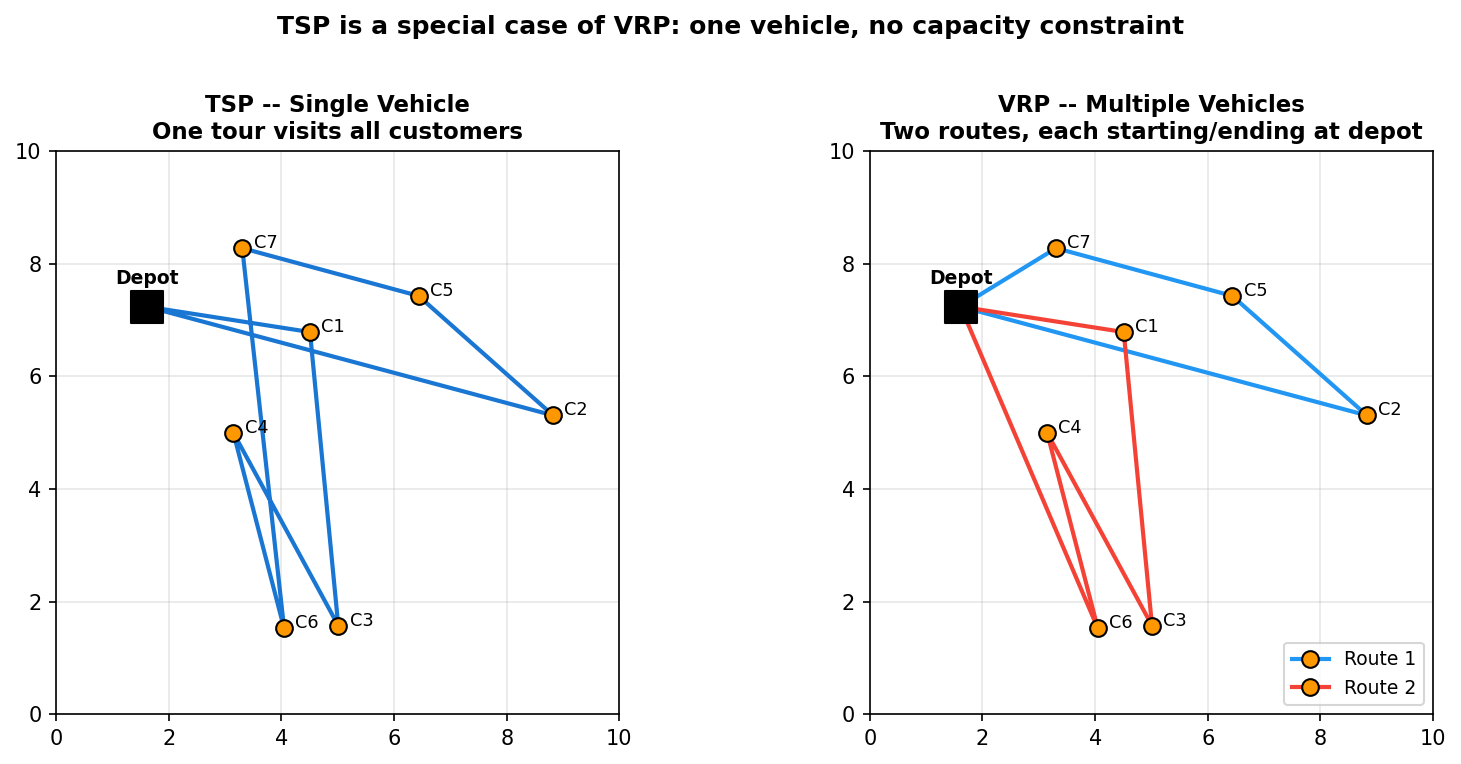
\includegraphics[width=0.70\linewidth]{tsp_vs_vrp.png}
\end{center}

\textbf{VRP reduces to TSP when:} there is only one vehicle ($K=1$) and no capacity
constraint ($Q = \infty$, infinity, meaning capacity is unlimited).  In this case, the
single vehicle must visit all customers in the cheapest order --- this is exactly
the TSP.  Since TSP is NP-hard, the VRP is also NP-hard.

\framebreak

\textbf{TSP as a lower bound component:}
Because any VRP solution is a set of TSP tours (one per route), and because
the optimal TSP tour over all customers is a lower bound on VRP cost (ignoring
capacity), TSP bounds are widely used in VRP branch-and-bound algorithms.

\medskip
\textbf{Relationship to Bin Packing:}
The \emph{customer-to-vehicle assignment} subproblem in the VRP is analogous to
bin packing:
\begin{itemize}
  \item Each customer's demand $d_i$ is an \emph{item} with size $d_i$.
  \item Each vehicle of capacity $Q$ is a \emph{bin} of size $Q$.
  \item The problem: pack all demands into the minimum number of bins (vehicles)
        without exceeding bin capacity.
\end{itemize}
This \emph{bin packing lower bound} gives the minimum number of vehicles needed:
\[
  K^* \geq \left\lceil \frac{\sum_{i=1}^{n} d_i}{Q} \right\rceil
\]
where $\lceil \cdot \rceil$ is the ceiling function (rounds up to the nearest integer).
For example, with total demand $= 47$ and $Q = 10$, we need at least
$\lceil 47/10 \rceil = 5$ vehicles.

\begin{alertblock}{Why These Relationships Matter}
Understanding the connection to TSP and bin packing allows us to borrow algorithmic
ideas from both fields.  TSP algorithms provide good initial tours; bin-packing
heuristics provide good initial vehicle assignments.  Many VRP heuristics alternate
between these two subproblems.
\end{alertblock}

\end{frame}

% ============================================================
\section{1.6 Benchmark Instances}
% ============================================================

\begin{frame}[allowframebreaks]{1.6 Benchmark Instances}

Benchmarking is critical in VRP research: it allows fair comparison of algorithms
across research groups.  Two sets of benchmark instances have been most widely used.

\begin{block}{Solomon's Benchmark Instances (1987)}
Solomon proposed 56 benchmark instances for the VRPTW, each with $n=100$ customers.
They are grouped into six types by the spatial distribution of customers and the
tightness of time windows:
\begin{itemize}
  \item \textbf{C-type (Clustered):} Customers form distinct geographic clusters.
        Routes naturally follow cluster boundaries.
  \item \textbf{R-type (Random):} Customers are uniformly distributed at random.
        Routes have no obvious geographic structure.
  \item \textbf{RC-type (Random-Clustered):} A mix of clustered and random customers.
\end{itemize}
Within each type, instances \textbf{1} have tight time windows and small vehicle
capacity (forcing many short routes), while instances \textbf{2} have wide time
windows and large capacity (permitting few long routes).
\end{block}

\begin{center}
  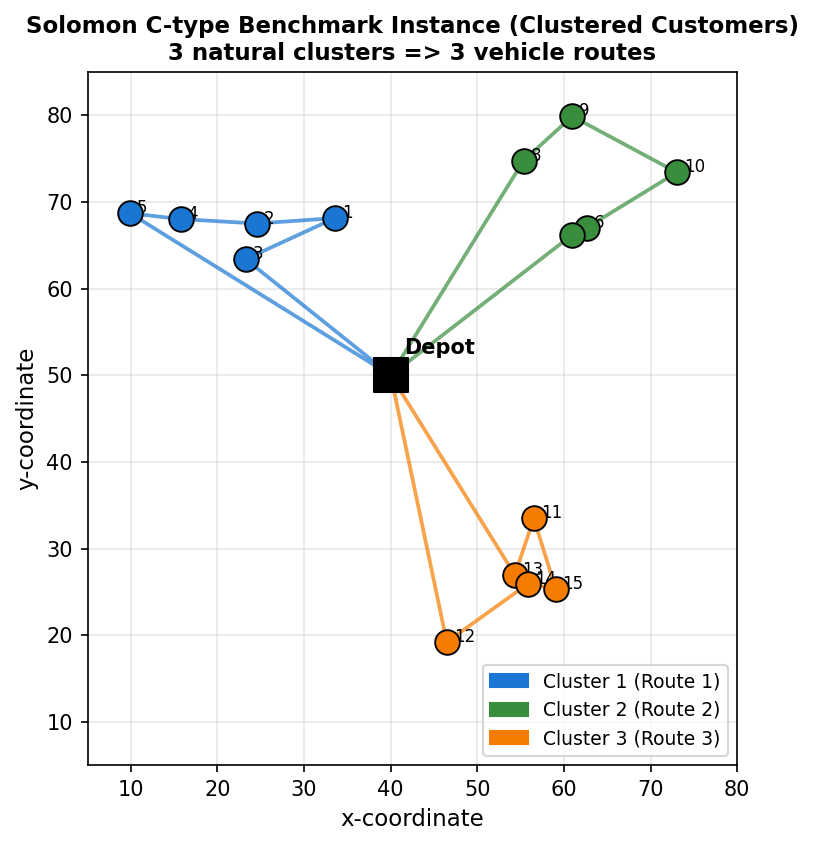
\includegraphics[width=0.55\linewidth]{solomon_instance.png}
\end{center}

\framebreak

\begin{block}{Christofides, Mingozzi, and Toth (CMT) Instances (1979)}
The CMT benchmark consists of 14 instances for the CVRP (no time windows), with
$n$ ranging from 50 to 199 customers.  These are the standard test bed for
capacitated VRP algorithms.  The instances are Euclidean (customer coordinates
are given, and distances are Euclidean).  Many best-known solutions for CMT
instances were found only decades after the instances were published, reflecting the
difficulty of the problem.
\end{block}

\textbf{Best-known solutions (BKS) and optimal solutions:}
\begin{itemize}
  \item For small CMT instances ($n \leq 75$), \emph{optimal} solutions are now known
        (found by exact branch-and-cut-and-price algorithms).
  \item For larger instances ($n \geq 100$), only \emph{best-known heuristic solutions}
        (BKS) are available.
  \item For Solomon's VRPTW instances, many optimal solutions are known for $n=100$
        instances, but the problems remain challenging.
\end{itemize}

\begin{alertblock}{Importance of Benchmarks}
Without standardised benchmarks, comparing two algorithms is scientifically
meaningless: one might solve easier instances, or use different computing resources.
Solomon's and CMT's instances have created a level playing field and enabled decades
of cumulative algorithmic progress.
\end{alertblock}

\end{frame}

% ============================================================
\section{1.7 Python: Implementing CVRP Tools}
% ============================================================

\begin{frame}[fragile]{Python: Computing CVRP Lower Bounds and Distances}

The following Python code implements basic CVRP utility functions: Euclidean distance,
bin-packing lower bound on number of vehicles, and the capacity-cut lower bound check.

\begin{lstlisting}[caption={CVRP utility functions (Python 3)}]
import numpy as np
import math

# -----------------------------------------------------------------
# Distance matrix from node coordinates
# -----------------------------------------------------------------
def euclidean_distance_matrix(coords):
    """
    coords: list of (x, y) tuples, coords[0] = depot
    Returns: n x n numpy array of Euclidean distances
    """
    n = len(coords)
    D = np.zeros((n, n))
    for i in range(n):
        for j in range(n):
            dx = coords[i][0] - coords[j][0]
            dy = coords[i][1] - coords[j][1]
            D[i][j] = math.sqrt(dx*dx + dy*dy)
    return D

# -----------------------------------------------------------------
# Bin-packing lower bound on number of vehicles
# -----------------------------------------------------------------
def bin_packing_lb(demands, capacity):
    """
    demands: list of customer demands (not including depot)
    capacity: vehicle capacity Q
    Returns: ceil(sum(demands) / capacity)
    """
    return math.ceil(sum(demands) / capacity)

# -----------------------------------------------------------------
# Route cost: total distance of a single route
# -----------------------------------------------------------------
def route_cost(route, dist_matrix):
    """
    route: list of node indices, e.g. [0, 2, 5, 3, 0]
    dist_matrix: n x n distance matrix
    Returns: total travel distance of the route
    """
    cost = 0.0
    for i in range(len(route) - 1):
        cost += dist_matrix[route[i]][route[i+1]]
    return cost
\end{lstlisting}

\end{frame}

\begin{frame}[fragile]{Python: Nearest Neighbour Heuristic for CVRP}

The \textbf{Nearest Neighbour (NN) heuristic} is the simplest construction heuristic
for CVRP.  Starting from the depot, it repeatedly adds the nearest unvisited customer
that does not violate the capacity constraint.  When no more customers can be added,
the vehicle returns to the depot and a new route begins.

The NN heuristic is fast ($O(n^2)$ time) but typically gives solutions 20--30\% above
optimal.  It is often used as a starting point for more sophisticated local search.

\begin{lstlisting}[caption={Nearest Neighbour heuristic for CVRP}]
def nearest_neighbour_cvrp(coords, demands, capacity):
    """
    coords : list of (x,y), coords[0] = depot
    demands: list of demands, demands[0] = 0 (depot)
    capacity: vehicle capacity Q
    Returns : list of routes (each route is a list of node indices)
    """
    D = euclidean_distance_matrix(coords)
    n = len(coords)
    unvisited = set(range(1, n))   # customer indices
    routes = []

    while unvisited:
        route   = [0]              # start at depot
        load    = 0.0

        while True:
            current = route[-1]
            # Find nearest unvisited customer that fits
            best, best_dist = None, float('inf')
            for j in unvisited:
                if load + demands[j] <= capacity:
                    if D[current][j] < best_dist:
                        best, best_dist = j, D[current][j]
            if best is None:
                break              # no feasible customer -> close route
            route.append(best)
            load += demands[best]
            unvisited.remove(best)

        route.append(0)            # return to depot
        routes.append(route)

    return routes

# ----- Example ---------------------------------------------------
coords  = [(5,5),(2,7),(1,4),(3,2),(7,2),(8,4),(8,7)]  # depot + 6 cust
demands = [0,    3,    4,    3,    4,    3,    3    ]
Q = 10
routes = nearest_neighbour_cvrp(coords, demands, Q)
for i, r in enumerate(routes):
    print(f"Route {i+1}: {r}, cost = {route_cost(r, euclidean_distance_matrix(coords)):.2f}")
\end{lstlisting}

\end{frame}

\begin{frame}[fragile]{Python: Clarke-Wright Savings Algorithm}

The \textbf{Clarke-Wright Savings Algorithm} (Clarke and Wright, 1964) is a classic
construction heuristic that builds routes by merging two initially separate ``spoke''
routes into a combined route whenever doing so yields a positive \emph{saving}.

\medskip
\textbf{Intuition.}
If every customer were served by a separate vehicle (spoke routes: depot $\to i \to$ depot),
the total cost would be $\sum_i 2 c_{0i}$ (twice the depot-to-customer distance for each
customer, where $c_{0i}$ is the cost from depot to customer $i$).
Merging customers $i$ and $j$ into one route (depot $\to i \to j \to$ depot) saves:
\[
  s(i,j) = c_{0i} + c_{0j} - c_{ij}
\]
A positive $s(i,j)$ means combining $i$ and $j$ into one route is cheaper than serving
them separately.  The algorithm merges routes in decreasing order of saving.

\begin{lstlisting}[caption={Clarke-Wright Savings Algorithm}]
def clarke_wright_savings(coords, demands, capacity):
    D = euclidean_distance_matrix(coords)
    n = len(coords)
    depot = 0

    # Compute all savings s(i,j) = d(0,i) + d(0,j) - d(i,j)
    savings = []
    for i in range(1, n):
        for j in range(1, n):
            if i < j:
                s = D[depot][i] + D[depot][j] - D[i][j]
                savings.append((s, i, j))
    savings.sort(reverse=True)   # sort by saving, largest first

    # Initialise: each customer on its own spoke route
    # route_of[i] = index of route containing customer i
    routes  = [[depot, i, depot] for i in range(1, n)]
    route_of = {i: i-1 for i in range(1, n)}
    load_of = {i-1: demands[i] for i in range(1, n)}

    def first_customer(route): return route[1]
    def last_customer(route):  return route[-2]

    for s, i, j in savings:
        ri = route_of.get(i)
        rj = route_of.get(j)
        if ri is None or rj is None: continue
        if ri == rj: continue   # already on same route
        # Merge only if i is at end of ri and j is at start of rj
        if (last_customer(routes[ri]) == i and
                first_customer(routes[rj]) == j and
                load_of[ri] + load_of[rj] <= capacity):
            # Merge: remove depot from end of ri and start of rj
            merged = routes[ri][:-1] + routes[rj][1:]
            routes[ri] = merged
            routes[rj] = None
            new_load = load_of[ri] + load_of[rj]
            load_of[ri] = new_load
            # Update route_of for all customers in rj
            for node in routes[ri]:
                if node != depot:
                    route_of[node] = ri

    return [r for r in routes if r is not None]
\end{lstlisting}

\end{frame}

\begin{frame}[fragile]{Python: 2-opt Local Search for Route Improvement}

The \textbf{2-opt} local search algorithm improves a single route by repeatedly
removing two edges and reconnecting the route in the only other way that maintains
a valid tour.  It is the simplest and most widely used VRP improvement heuristic.

\begin{lstlisting}[caption={2-opt local search for route improvement}]
def two_opt(route, dist_matrix):
    """
    Improve a single route using 2-opt swaps.
    route: list of nodes including depot at start and end, e.g. [0,2,3,5,0]
    Returns: improved route and its cost
    """
    best = route[:]
    improved = True
    while improved:
        improved = False
        for i in range(1, len(best) - 2):
            for j in range(i + 1, len(best) - 1):
                # Try reversing the segment best[i:j+1]
                new_route = best[:i] + best[i:j+1][::-1] + best[j+1:]
                old_cost  = route_cost(best,      dist_matrix)
                new_cost  = route_cost(new_route, dist_matrix)
                if new_cost < old_cost - 1e-9:
                    best = new_route
                    improved = True
    return best

# ---- Example: improve a route --------------------------------
D = euclidean_distance_matrix(
        [(5,5),(2,7),(1,4),(3,2),(7,2),(8,4),(8,7)])
route = [0, 1, 3, 2, 4, 5, 6, 0]
print(f"Before 2-opt: cost = {route_cost(route, D):.2f}")
improved = two_opt(route, D)
print(f"After  2-opt: cost = {route_cost(improved, D):.2f}")
print(f"Improved route: {improved}")
\end{lstlisting}

\medskip
The 2-opt algorithm runs in $O(n^2)$ per iteration and typically converges in a
small number of passes.  For a route of length $k$, there are $\binom{k-1}{2}$
possible 2-opt moves, so one full pass has at most $O(k^2)$ evaluations.

\end{frame}

% ============================================================
\section{1.8 Key Takeaways and Chapter Summary}
% ============================================================

\begin{frame}[allowframebreaks]{Chapter 1 Summary: Key Takeaways}

This chapter has introduced the full landscape of vehicle routing problems.  The
following points summarise the most important concepts.

\begin{block}{1. The Core Problem: CVRP}
The Capacitated VRP is the foundation of the entire field.  It asks: given $n$
customers with demands, $K$ vehicles of capacity $Q$, and a depot, find the
minimum-cost set of routes that covers every customer exactly once without
violating capacity.  The problem is NP-hard (it includes TSP as a special case).
\end{block}

\begin{block}{2. Mathematical Models}
Two key formulations exist:
\begin{itemize}
  \item \emph{Arc-flow models} (MTZ-style): use binary variables $x_{ij}$ and
        auxiliary variables $u_i$ for subtour elimination.
  \item \emph{Set-partitioning model}: enumerate all feasible routes; select the
        minimum-cost covering subset.  Solved via column generation.
\end{itemize}
\end{block}

\begin{block}{3. The VRP Family}
Real-world variants include:
VRPTW (time windows), PDP/PDPTW (pickup and delivery), SVRP (stochastic),
DVRP (dynamic), VRPP (profits), SDVRP (split deliveries), HVRP (heterogeneous fleet),
PVRP (periodic), MDVRP (multi-depot).
Each adds one or more constraints or relaxations to the basic CVRP.
\end{block}

\framebreak

\begin{block}{4. Relationship to TSP and Bin Packing}
\begin{itemize}
  \item VRP with one vehicle and no capacity = TSP.
  \item Customer-to-vehicle assignment $\approx$ bin packing.
  \item Both relationships yield useful lower bounds and algorithmic ideas.
\end{itemize}
\end{block}

\begin{block}{5. Benchmarks}
\begin{itemize}
  \item \textbf{Christofides-Mingozzi-Toth (CMT)}: 14 CVRP instances,
        $n \in [50, 199]$; standard for capacitated routing.
  \item \textbf{Solomon (1987)}: 56 VRPTW instances, $n=100$; C/R/RC types;
        standard for time-window routing.
\end{itemize}
\end{block}

\begin{alertblock}{Final Takeaway}
The Vehicle Routing Problem is one of the most practically important optimisation
problems, with billions of dollars of potential savings in global logistics.  Its
mathematical richness --- combining graph theory, integer programming, and
combinatorial optimisation --- makes it a cornerstone of operations research.
Every logistics company, from last-mile delivery startups to global supply chains,
faces a VRP variant every single day.
\end{alertblock}

\end{frame}

% ============================================================
\section{Bibliography (Selected)}
% ============================================================

\begin{frame}[allowframebreaks]{Selected Bibliography}

The following references are among the most foundational works in the VRP literature,
as cited in Chapter 1 of Irnich, Toth, and Vigo (2014).

\medskip
\begin{thebibliography}{99}\small
\bibitem{BalQua64}
  M.L.~Balinski and R.E.~Quandt,
  \emph{On an integer program for a delivery problem},
  Operations Research, 12 (1964), pp.~300--304.

\bibitem{ClaWri64}
  G.~Clarke and J.W.~Wright,
  \emph{Scheduling of vehicles from a central depot to a number of delivery points},
  Operations Research, 12 (1964), pp.~568--581.

\bibitem{CMT79}
  N.~Christofides, A.~Mingozzi, and P.~Toth,
  \emph{The vehicle routing problem},
  in Combinatorial Optimisation, Wiley, 1979, pp.~315--338.

\bibitem{Sol87}
  M.M.~Solomon,
  \emph{Algorithms for the vehicle routing and scheduling problems with time window
  constraints},
  Operations Research, 35 (1987), pp.~254--265.

\bibitem{TotVig02}
  P.~Toth and D.~Vigo (eds.),
  \emph{The Vehicle Routing Problem},
  SIAM Monographs on Discrete Mathematics and Applications, SIAM, Philadelphia, 2002.

\bibitem{IrnTotVig14}
  S.~Irnich, P.~Toth, and D.~Vigo,
  \emph{The family of vehicle routing problems},
  Chapter~1 in: P.~Toth and D.~Vigo (eds.),
  \emph{Vehicle Routing: Problems, Methods, and Applications},
  2nd ed., SIAM, 2014.

\bibitem{LapNor87}
  G.~Laporte and Y.~Nobert,
  \emph{Exact algorithms for the vehicle routing problem},
  Annals of Discrete Mathematics, 31 (1987), pp.~147--184.

\bibitem{CorLap03}
  J.-F.~Cordeau and G.~Laporte,
  \emph{The dial-a-ride problem: Modeling and solution},
  Journal of the Operational Research Society, 58 (2003), pp.~293--307.

\bibitem{GenLapSeb92}
  M.~Gendreau, A.~Hertz, and G.~Laporte,
  \emph{New insertion and postoptimization procedures for the traveling salesman problem},
  Operations Research, 40 (1992), pp.~1086--1094.
\end{thebibliography}

\end{frame}

% ============================================================
\begin{frame}{}
  \begin{center}
    \Large\textbf{End of Chapter 1}\\[12pt]
    \normalsize The Family of Vehicle Routing Problems\\[8pt]
    \textit{Irnich, Toth, Vigo --- Vehicle Routing: Problems, Methods, and Applications, 2nd ed., SIAM 2014}
  \end{center}
\end{frame}

\end{document}
